\documentclass[10pt]{article}
\usepackage[margin=1in]{geometry}
\usepackage{graphicx}
\usepackage{microtype}
\usepackage[hidelinks]{hyperref}
\title{Calibrating Word-Level Confidence in Bangla Speech Recognition Across Regional Dialects}
\author{Ismail Hossain Polas \\\\ Jahangirnagar University \\\\ ismailhossainpolash@gmail.com}
\date{}
\begin{document}
\maketitle
\begin{abstract}

A transcription pipeline can send its least certain words to a human reviewer, but only if the model's word confidence means what it says. Bangla dialect benchmarks report error rates and nothing about confidence. We measure word-level confidence for four public Bangla recognisers (two Whisper-medium checkpoints, Whisper-large-v3 and an XLS-R CTC model) on 2,668 clips from 12 Bangladeshi regional dialects, and on 2,500 Standard Bangla clips from Common Voice. Raw confidence is overconfident on every model: mean confidence exceeds accuracy by 0.42 to 0.71, and per-region expected calibration error (ECE) is 0.42 to 0.71. A gradient-boosted calibrator over 12 decoding features, trained on the other dialects, brings ECE to between 0.023 and 0.051. A calibrator trained on Standard Bangla ranks dialect errors almost as well (AUROC down 0.020 to 0.024 on three of four models and 0.072 on the fourth) but is miscalibrated on the two Whisper-medium models (ECE 0.33 and 0.19, against 0.051 and 0.049 for a calibrator trained on other dialects). That failure grows with the gap in error rate between training and target speech, and about 100 labelled target words bring the three Whisper models to an ECE between 0.048 and 0.070, whereas estimating the error rate without labels does not help. Even after calibration, at most 0.1\% of dialect words reach a confidence of 0.9, so confidence-based review has limited reach on these models.


\end{abstract}

\section{Introduction}

Word-level confidence is what lets a speech pipeline decide which words a person should check~\cite{Oneata2021,Qiu2021}. A call-centre transcription service in Bangladesh would use it that way, and it would meet speech that differs from the Standard Bangla in most training data.


Recent Bangla work documents that difference but not its consequence for confidence. Ben-10 benchmarks Whisper, wav2vec 2.0, a Conformer and Google ASR on ten regional dialects and finds that all of them struggle, zero-shot and fine-tuned~\cite{Dipto2025}. RegSpeech12 adds spontaneous speech from twelve regions~\cite{Hassan2025}, and BanglaTalk evaluates a dialect-aware recogniser on it~\cite{Hasan2025}. These papers report word and character error rates. Work on confidence, meanwhile, has measured calibration under additive noise~\cite{Huo2025}, out-of-domain English text domains~\cite{Li2022} and a single English accent~\cite{Jia2026}, and has related Whisper's confidence to a language's training data~\cite{Liang2025}. In the literature we searched (arXiv and the ACL and ISCA archives, through October 2026), we found no study of word-level confidence on dialect speech in any language.


We ask two questions. First, how miscalibrated is the confidence of public Bangla recognisers on regional dialects? Second, does a calibrator fitted on one kind of Bangla speech, in particular Standard Bangla, remain usable on another? We answer both on 12 Bangladeshi dialects with four models, using a 12-feature gradient-boosted calibrator, Platt scaling and the raw model probabilities.


Our findings are these:


\begin{enumerate}

\item Raw word confidence is badly overconfident on all four models (mean confidence exceeds accuracy by 0.42 to 0.71; per-region ECE 0.42 to 0.71), and a calibrator trained on the other dialects reduces it to 0.023 to 0.051 on a held-out dialect.

\item A calibrator trained on Standard Bangla keeps most of its ranking ability on dialects but loses calibration on the Whisper-medium models; the loss scales with the error-rate gap between source and target.

\item About 100 labelled target words recalibrate the Whisper models to an ECE of 0.048 to 0.070, whereas label-free estimation of the target error rate does not help.

\item Calibrated confidence rarely exceeds 0.9 on dialect speech, which bounds how many words any confidence threshold can accept.

\end{enumerate}

\section{Related work}

\begin{table}[htb]
\centering
\par\noindent\begin{minipage}{\linewidth}\small Table R. Closest prior work. ``Dialect speech'' means the evaluation speech is a regional variety.\end{minipage}\par\smallskip
\footnotesize
\begin{tabular}{p{3.4cm}p{2.9cm}p{4.6cm}cc}
\hline
\textbf{Paper} & \textbf{Confidence or calibration measured} & \textbf{Shift studied} & \textbf{Dialect speech} & \textbf{Bangla} \\ \hline
Li et al. 2022 & word/token, yes & text and acoustic domain (TED-LIUM, Switchboard) & no & no \\
Aggarwal et al. 2025 & word, yes & eight out-of-domain sets & no & no \\
Huo et al. 2025 & token, yes & additive noise & no & no \\
Jia and Van hamme 2026 & token and word, yes & Common Voice, US accent only & no & no \\
Liang et al. 2025 & sub-token probabilities & language resource level & no & no \\
Ballier et al. 2024 & ECE, yes & three languages & no & no \\
Dipto 2025; Hassan 2025; Hasan 2025 & no & regional dialects & yes & yes \\
This paper & word, yes & Standard Bangla and 12 dialects & yes & yes \\
\hline\end{tabular}
\end{table}


Confidence for end-to-end recognisers is usually estimated by a small module over decoder features. Qiu et al. learn word-level confidence for word-piece models~\cite{Qiu2021}, and Oneata et al. evaluate several estimators on end-to-end systems~\cite{Oneata2021}. Laptev and Ginsburg propose entropy-based scores that need no training~\cite{Laptev2022}. Naowarat et al. extend the idea to CTC models and add neighbouring words as context~\cite{Naowarat2023}. None of these papers evaluates on dialect or accent speech.


Several studies address distribution shift. Li et al. show that a confidence module trained in-domain degrades out of domain and repair it with pseudo-transcriptions and an extra language model~\cite{Li2022}. Aggarwal et al. fine-tune Whisper to emit word confidence and report gains on eight out-of-domain datasets over a feature-based module~\cite{Aggarwal2025}. Huo et al. find that Whisper's overconfident errors rise at low signal-to-noise ratio and correct them with temperature scaling on selected tokens~\cite{Huo2025}. Jia and Van hamme score tokens from beam-search ranks and test on US-accented Common Voice~\cite{Jia2026}. Liang et al. probe Whisper's sub-token probabilities across languages~\cite{Liang2025}, and Ballier et al. relate calibration to training data in three languages~\cite{Ballier2024}. The shift in each case is noise, text domain, language or a single accent. Dialect speech, where both the acoustics and the vocabulary change, is not among them.


For Bangla, the corpora and benchmarks above supply error rates only~\cite{Dipto2025,Hassan2025,Hasan2025}. Among the Bangla speech papers we reviewed, none mentions confidence or calibration.


\section{Data and models}

\textbf{Speech.} The RegSpeech12 test split has 2,132 clips of spontaneous speech labelled with one of 12 regions~\cite{Hassan2025}. Its transcripts are written in dialectal spelling, for example ``taha'' where Standard Bangla writes ``taka'' (romanised). Comilla and Noakhali do not appear in Ben-10, so the regional checkpoint cannot have trained on them, and the test split holds only 32 and 28 of their clips. We therefore add all their training and validation clips (286 and 250), which gives 2,668 clips (Table 0). Their transcripts show no overlap with Ben-10 in any split (Section below), so this use of training and validation clips adds no leakage for the regional checkpoint. No clip is used both to fit and to evaluate a calibrator: leave-one-dialect-out holds out whole regions, Standard-to-dialect training uses Common Voice only, and recalibration splits by utterance.


\begin{table}[htb]
\centering
\par\noindent\begin{minipage}{\linewidth}\small Table 0. Clips per region used for evaluation (test split plus, for Comilla and Noakhali, all training and validation clips)\end{minipage}\par\smallskip
\small
\resizebox{\ifdim\width>\linewidth\linewidth\else\width\fi}{!}{
\begin{tabular}{lcccc}
\hline
\textbf{Region} & \textbf{Test clips} & \textbf{Added from train/valid} & \textbf{Total} & \textbf{Used for regional checkpoint} \\ \hline
barishal & 101 & 0 & 101 & yes \\
chittagong & 176 & 0 & 176 & yes \\
comilla & 32 & 286 & 318 & yes \\
habiganj & 117 & 0 & 117 & yes \\
kishoreganj & 205 & 0 & 205 & yes \\
narail & 186 & 0 & 186 & yes \\
narsingdi & 137 & 0 & 137 & yes \\
noakhali & 28 & 250 & 278 & yes \\
rangpur & 130 & 0 & 130 & no (test text overlaps Ben-10) \\
sandwip & 131 & 0 & 131 & yes \\
sylhet & 762 & 0 & 762 & yes \\
tangail & 127 & 0 & 127 & yes \\
Total & 2132 & 536 & 2668 &  \\
\hline\end{tabular}}
\end{table}


For Standard Bangla we draw 2,500 clips at random (seed 0) from the 9,230-clip test split of Common Voice 13 Bengali, which is read speech in short clips (mean 6.4 s, against 16.9 s for the dialect clips).


\textbf{Overlap with Ben-10.} The regional Whisper checkpoint comes from the Ben-10 project, so we compared transcripts. In nine regions, 84.7\% to 98.8\% of RegSpeech12 training clips and 92.7\% to 100\% of validation clips share a six-word sequence with Ben-10 text. The test split is clean apart from Rangpur, where 93.8\% of clips overlap (other regions: 0\% to 4.0\%). Apart from Comilla and Noakhali, we therefore use only the test split for dialects, and we drop Rangpur for the regional checkpoint (so that checkpoint is evaluated on 11 regions). Neither corpus gives speaker identity, so speaker overlap is unknown.


\textbf{Models.} We use two Whisper-medium checkpoints released by BengaliAI, one for Standard Bangla (Std) and one for regional speech (Reg), Whisper-large-v3 used zero-shot with the language set to Bangla, and a public XLS-R-300M CTC checkpoint fine-tuned for Bangla. Decoding is greedy with clips cut at 30 seconds and at most 200 new tokens.


\section{Method}

\textbf{Word confidence features.} For the Whisper models we run the generated sequence back through the decoder with the standard prompt and take the probability of each emitted token. Tokens are grouped into words at the leading-space marker. Each word gets 12 features. Five are probability statistics: the mean, minimum, first and last token probability, and the mean log-probability. Three describe the full-vocabulary distribution: mean entropy, maximum entropy and the mean margin between the top two candidates. Four are positional: the token count, the relative position in the utterance, the length of the hypothesis in words and the character length. For the CTC model we use the same statistics over the frame-level maximum probabilities of the emitted, non-blank frames, grouped by the word delimiter.


\textbf{Error labels.} We remove angle-bracket tags and punctuation from references and hypotheses, align them at word level by edit distance, and call a hypothesis word an error if it is substituted or inserted. Deleted reference words are not scored, so the error rates we report for calibration are shares of hypothesis words, not word error rates; Table 1 gives conventional WER (substitutions, deletions and insertions over reference words) alongside. The strict label counts any mismatch. The lenient label counts a substitution as correct when its character edit distance is at most 0.34 of the longer word, which forgives many spelling variants.


\textbf{Calibrators.} We compare the raw mean token probability and raw minimum token probability, Platt scaling on the logit of the mean probability, and a gradient-boosted classifier (200 iterations, learning rate 0.08, 15 leaves) over the 12 features. Each outputs the probability that the word is correct.


\textbf{Protocols.} In leave-one-dialect-out evaluation the calibrator is trained on the words of the other 11 dialects and scored on the held-out one. An in-distribution control trains on a random 80\% of utterances from all dialects and scores the rest. For Standard-to-dialect transfer the calibrator is trained only on the Common Voice words. For recalibration we draw whole utterances from the target dialect until they supply n labelled words, fit Platt scaling to the source calibrator's output on them, and score the remaining utterances, repeating 20 times per dialect. We also test two error-rate adjustments: one shifts the log-odds by the difference between the target's and source's error rates, using the true target rate (an upper bound), and one estimates that rate without labels by expectation-maximisation.


\textbf{Metrics.} ECE uses 15 equal-width bins. We report it per region and average over regions weighted by word count, because pooling across regions lets opposite errors cancel (pooled ECE is 0.003 to 0.006 for the dialect-trained GBM in both leave-one-dialect-out and the control, which hides regional error). AUROC measures how well confidence separates errors from correct words. Pooled bootstrap intervals resample utterances 100 times.


\section{Results}

\subsection{Raw confidence is overconfident}

\begin{table}[htb]
\centering
\par\noindent\begin{minipage}{\linewidth}\small Table 1. Error rates by speech type and raw confidence. WER = (substitutions + deletions + insertions) / reference words. Error share = wrong hypothesis words / hypothesis words, the quantity the calibrators predict. Share = error share; dial. = dialects; Conf. = mean raw token-probability confidence on dialect words; Gap = Conf. minus observed accuracy (positive = overconfident); ECE and AUROC use the raw mean (mean) or minimum (min) token probability, AUROC for the mean.\end{minipage}\par\smallskip
\small
\resizebox{\ifdim\width>\linewidth\linewidth\else\width\fi}{!}{
\begin{tabular}{lccccccccc}
\hline
\textbf{Model} & \textbf{WER CV} & \textbf{WER dial.} & \textbf{Share CV} & \textbf{Share dial.} & \textbf{Conf.} & \textbf{Gap} & \textbf{ECE mean} & \textbf{ECE min} & \textbf{AUROC} \\ \hline
Whisper-med (Std) & 0.10 & 0.80 & 0.09 & 0.68 & 0.91 & +0.59 & 0.59 & 0.48 & 0.746 \\
Whisper-med (Reg) & 0.14 & 0.72 & 0.13 & 0.62 & 0.80 & +0.42 & 0.42 & 0.21 & 0.716 \\
Whisper-large-v3 & 0.88 & 0.97 & 0.77 & 0.87 & 0.83 & +0.71 & 0.71 & 0.41 & 0.615 \\
XLS-R (CTC) & 0.50 & 0.94 & 0.44 & 0.83 & 0.78 & +0.61 & 0.61 & 0.42 & 0.801 \\
\hline\end{tabular}}
\end{table}


Table 1 shows that every model claims far more accuracy than it has. For the Standard Whisper-medium checkpoint, 68\% of dialect hypothesis words are wrong (WER 0.80), yet its mean word confidence is 0.91, a signed gap of +0.59 above its accuracy of 0.32. The gap is positive on all four models (+0.42 to +0.71) and in every region (Table 9, Figure 1), so the ECE reflects overconfidence and not merely mismatch. Minimum token probability gives a lower ECE on every model, down to 0.21 on the regional checkpoint, but remains overconfident (gaps +0.21 to +0.48).


\begin{figure}[htb]\centering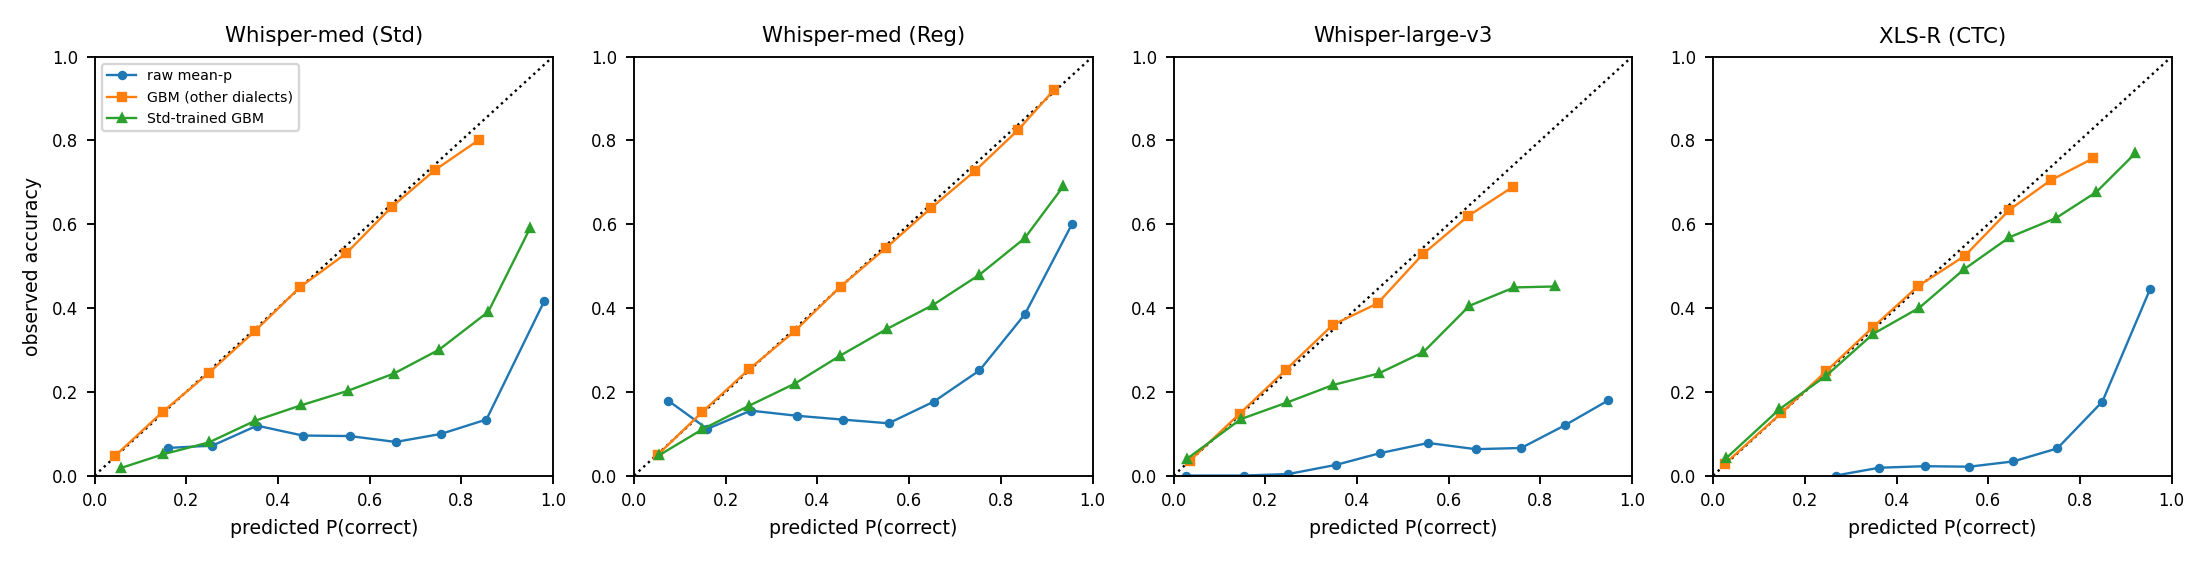
\includegraphics[width=\linewidth]{fig_reliability.png}\par\smallskip\begin{minipage}{\linewidth}\small Figure 1. Reliability curves on dialect words: observed accuracy against predicted probability of being correct, for the raw mean token probability, a GBM trained on other dialects and a GBM trained on Standard Bangla (Common Voice). Points under the diagonal are overconfident. Bins with fewer than 30 words are omitted.\end{minipage}\end{figure}


\begin{table}[htb]
\centering
\par\noindent\begin{minipage}{\linewidth}\small Table 9. Signed gap (mean predicted probability of correct minus accuracy; pooled over dialect words, with the range over regions) and Brier score\end{minipage}\par\smallskip
\small
\resizebox{\ifdim\width>\linewidth\linewidth\else\width\fi}{!}{
\begin{tabular}{lccc}
\hline
\textbf{Model} & \textbf{Estimator} & \textbf{Signed gap (region range)} & \textbf{Brier} \\ \hline
Whisper-med (Std) & raw mean-p & +0.590 (+0.35 to +0.72) & 0.547 \\
Whisper-med (Std) & raw min-p & +0.476 (+0.31 to +0.54) & 0.420 \\
Whisper-med (Std) & GBM, other dialects & +0.003 ($-$0.14 to +0.07) & 0.168 \\
Whisper-med (Std) & GBM, Standard-trained & +0.327 (+0.21 to +0.37) & 0.298 \\
Whisper-med (Reg) & raw mean-p & +0.415 (+0.22 to +0.51) & 0.380 \\
Whisper-med (Reg) & raw min-p & +0.205 (+0.08 to +0.26) & 0.246 \\
Whisper-med (Reg) & GBM, other dialects & +0.003 ($-$0.14 to +0.07) & 0.184 \\
Whisper-med (Reg) & GBM, Standard-trained & +0.186 (+0.08 to +0.24) & 0.235 \\
Whisper-large-v3 & raw mean-p & +0.707 (+0.59 to +0.77) & 0.620 \\
Whisper-large-v3 & raw min-p & +0.402 (+0.34 to +0.46) & 0.319 \\
Whisper-large-v3 & GBM, other dialects & $-$0.000 ($-$0.10 to +0.07) & 0.091 \\
Whisper-large-v3 & GBM, Standard-trained & +0.052 ($-$0.04 to +0.10) & 0.109 \\
XLS-R (CTC) & raw mean-p & +0.611 (+0.52 to +0.66) & 0.492 \\
XLS-R (CTC) & raw min-p & +0.415 (+0.35 to +0.45) & 0.289 \\
XLS-R (CTC) & GBM, other dialects & $-$0.000 ($-$0.05 to +0.03) & 0.102 \\
XLS-R (CTC) & GBM, Standard-trained & +0.005 ($-$0.05 to +0.05) & 0.108 \\
\hline\end{tabular}}
\end{table}


AUROC of the raw scores is 0.62 to 0.80, with Whisper-large-v3 weakest. Under the lenient label the pooled ECE of the raw mean probability falls by 0.05 to 0.12 and stays between 0.30 and 0.65.


\subsection{A calibrator trained on other dialects transfers}

\begin{table}[htb]
\centering
\par\noindent\begin{minipage}{\linewidth}\small Table 2. Calibrators trained on the other dialects (leave-one-dialect-out), per-region ECE / AUROC (n-weighted over 12 regions, strict labels)\end{minipage}\par\smallskip
\small
\resizebox{\ifdim\width>\linewidth\linewidth\else\width\fi}{!}{
\begin{tabular}{lcccc}
\hline
\textbf{Model} & \textbf{raw mean-p} & \textbf{raw min-p} & \textbf{Platt (mean-p)} & \textbf{GBM (12 features)} \\ \hline
Whisper-med (Std) & 0.590 / 0.746 & 0.476 / 0.753 & 0.060 / 0.744 & 0.051 / 0.782 \\
Whisper-med (Reg) & 0.415 / 0.716 & 0.206 / 0.720 & 0.071 / 0.716 & 0.049 / 0.767 \\
Whisper-large-v3 & 0.707 / 0.615 & 0.413 / 0.598 & 0.049 / 0.615 & 0.035 / 0.823 \\
XLS-R (CTC) & 0.611 / 0.801 & 0.415 / 0.799 & 0.048 / 0.801 & 0.023 / 0.851 \\
\hline\end{tabular}}
\end{table}


\begin{table}[htb]
\centering
\par\noindent\begin{minipage}{\linewidth}\small Pooled (single ECE over all held-out words) GBM LODO vs in-distribution 5-fold control (ECE / AUROC)\end{minipage}\par\smallskip
\small
\resizebox{\ifdim\width>\linewidth\linewidth\else\width\fi}{!}{
\begin{tabular}{lcc}
\hline
\textbf{Model} & \textbf{LODO pooled} & \textbf{in-distribution} \\ \hline
Whisper-med (Std) & 0.007 / 0.793 & 0.006 / 0.799 \\
Whisper-med (Reg) & 0.005 / 0.779 & 0.005 / 0.783 \\
Whisper-large-v3 & 0.005 / 0.825 & 0.004 / 0.830 \\
XLS-R (CTC) & 0.005 / 0.862 & 0.007 / 0.864 \\
\hline\end{tabular}}
\end{table}


Table 2 shows that the 12-feature GBM trained on the other 11 dialects reaches a per-region ECE of 0.023 to 0.051 and an AUROC of 0.767 to 0.851. Platt scaling alone fixes most of the calibration (0.048 to 0.071) but leaves AUROC at the raw level, so the extra ranking ability comes from the other features. The pooled leave-one-dialect-out result is within 0.006 AUROC of the in-distribution control for every model, and the clip-level bootstrap intervals in Table 8 are narrow (for the Standard checkpoint, ECE 0.051 [0.048, 0.055] and AUROC 0.782 [0.778, 0.787]). The calibrated estimators are close to unbiased on average (pooled signed gap within 0.003 of zero on all four models, Table 9), although the gap ranges from $-$0.14 to +0.07 across regions, and their Brier scores are 0.09 to 0.18 against 0.25 to 0.62 for the raw probabilities. The intervals are bias-corrected percentile intervals: ECE is biased upward under resampling, and plain percentile intervals missed the point estimate in one case. Calibration therefore transfers between these 12 dialects. Table 6 checks whether this depends on the hand-built features.


\subsection{Standard Bangla to dialects: ranking holds, calibration does not}

\begin{table}[htb]
\centering
\par\noindent\begin{minipage}{\linewidth}\small Table 3. Calibrator trained on Standard Bangla (Common Voice) applied to the dialects (per-region ECE / AUROC, n-weighted over regions, strict)\end{minipage}\par\smallskip
\small
\resizebox{\ifdim\width>\linewidth\linewidth\else\width\fi}{!}{
\begin{tabular}{lccccc}
\hline
\textbf{Model} & \textbf{raw mean-p} & \textbf{Platt} & \textbf{GBM} & \textbf{GBM + oracle shift} & \textbf{GBM, dialect-trained} \\ \hline
Whisper-med (Std) & 0.590 / 0.746 & 0.349 / 0.744 & 0.327 / 0.758 & 0.115 / 0.758 & 0.051 / 0.782 \\
Whisper-med (Reg) & 0.415 / 0.716 & 0.228 / 0.716 & 0.187 / 0.746 & 0.167 / 0.746 & 0.049 / 0.767 \\
Whisper-large-v3 & 0.707 / 0.615 & 0.100 / 0.615 & 0.071 / 0.751 & 0.038 / 0.751 & 0.035 / 0.823 \\
XLS-R (CTC) & 0.611 / 0.801 & 0.103 / 0.801 & 0.035 / 0.831 & 0.112 / 0.831 & 0.023 / 0.851 \\
\hline\end{tabular}}
\end{table}


Table 3 compares calibrators trained on Standard Bangla with the dialect-trained ones. On the two Whisper-medium models the Standard-trained GBM has per-region ECE of 0.327 and 0.187, against 0.051 and 0.049 when trained on other dialects (paired differences 0.275 and 0.137, Table 8), and it stays overconfident (signed gap +0.33 and +0.19, Table 9). Platt scaling is no better (Table 3). Ranking degrades much less: AUROC falls by 0.024 (Std), 0.022 (Reg) and 0.020 (XLS-R), against 0.072 for Whisper-large-v3 (Table 8). All GBM fits are deterministic (early stopping is disabled), so Tables 3 and 8 report the same fits. The intervals in Table 8 reflect resampling of evaluation clips with the fitted calibrators held fixed; they do not include uncertainty from fitting the calibrator. The reverse direction fares no better (Table 3b).


\begin{table}[htb]
\centering
\par\noindent\begin{minipage}{\linewidth}\small Table 8. Per-region ECE and AUROC with 95\% bootstrap intervals (clips resampled within region, 1000 replicates; regions weighted by word count). The last row is the paired difference, Standard-trained minus other-dialect-trained GBM (ECE) and the reverse (AUROC). Bias-corrected percentile intervals (ECE is biased upward under resampling); they reflect clip resampling with the fitted calibrators held fixed.\end{minipage}\par\smallskip
\small
\resizebox{\ifdim\width>\linewidth\linewidth\else\width\fi}{!}{
\begin{tabular}{lccc}
\hline
\textbf{Model} & \textbf{Estimator} & \textbf{ECE [95\% CI]} & \textbf{AUROC [95\% CI]} \\ \hline
Whisper-med (Std) & raw mean-p & 0.590 [0.585, 0.596] & 0.746 [0.742, 0.751] \\
Whisper-med (Std) & Platt, other dialects & 0.060 [0.056, 0.064] & 0.744 [0.740, 0.749] \\
Whisper-med (Std) & GBM, other dialects & 0.051 [0.048, 0.055] & 0.782 [0.778, 0.787] \\
Whisper-med (Std) & GBM, Standard-trained & 0.327 [0.322, 0.331] & 0.758 [0.754, 0.763] \\
Whisper-med (Std) & paired difference & 0.275 [0.269, 0.281] & 0.024 [0.021, 0.027] \\
Whisper-med (Reg) & raw mean-p & 0.415 [0.410, 0.420] & 0.716 [0.711, 0.720] \\
Whisper-med (Reg) & Platt, other dialects & 0.071 [0.067, 0.076] & 0.716 [0.711, 0.720] \\
Whisper-med (Reg) & GBM, other dialects & 0.049 [0.045, 0.053] & 0.767 [0.764, 0.771] \\
Whisper-med (Reg) & GBM, Standard-trained & 0.187 [0.183, 0.191] & 0.746 [0.742, 0.750] \\
Whisper-med (Reg) & paired difference & 0.137 [0.132, 0.142] & 0.022 [0.020, 0.023] \\
Whisper-large-v3 & raw mean-p & 0.707 [0.700, 0.713] & 0.615 [0.603, 0.626] \\
Whisper-large-v3 & Platt, other dialects & 0.049 [0.044, 0.054] & 0.615 [0.603, 0.626] \\
Whisper-large-v3 & GBM, other dialects & 0.035 [0.031, 0.038] & 0.823 [0.815, 0.831] \\
Whisper-large-v3 & GBM, Standard-trained & 0.071 [0.066, 0.075] & 0.751 [0.741, 0.761] \\
Whisper-large-v3 & paired difference & 0.036 [0.031, 0.042] & 0.072 [0.065, 0.079] \\
XLS-R (CTC) & raw mean-p & 0.611 [0.607, 0.616] & 0.801 [0.794, 0.808] \\
XLS-R (CTC) & Platt, other dialects & 0.048 [0.044, 0.051] & 0.801 [0.794, 0.808] \\
XLS-R (CTC) & GBM, other dialects & 0.023 [0.020, 0.026] & 0.851 [0.846, 0.856] \\
XLS-R (CTC) & GBM, Standard-trained & 0.035 [0.032, 0.039] & 0.831 [0.825, 0.836] \\
XLS-R (CTC) & paired difference & 0.013 [0.010, 0.016] & 0.020 [0.017, 0.023] \\
\hline\end{tabular}}
\end{table}


\begin{table}[htb]
\centering
\par\noindent\begin{minipage}{\linewidth}\small Table 3b. Calibrator trained on all dialects, applied to Standard Bangla (Common Voice): ECE / AUROC (strict)\end{minipage}\par\smallskip
\small
\resizebox{\ifdim\width>\linewidth\linewidth\else\width\fi}{!}{
\begin{tabular}{lcc}
\hline
\textbf{Model} & \textbf{Platt} & \textbf{GBM} \\ \hline
Whisper-med (Std) & 0.342 / 0.793 & 0.352 / 0.773 \\
Whisper-med (Reg) & 0.203 / 0.818 & 0.262 / 0.773 \\
Whisper-large-v3 & 0.108 / 0.767 & 0.071 / 0.819 \\
XLS-R (CTC) & 0.087 / 0.801 & 0.159 / 0.782 \\
\hline\end{tabular}}
\end{table}


XLS-R is the exception to the ECE pattern: its Standard-trained GBM reaches 0.035 with no error-rate correction.


The error rate may account for much of this. Common Voice error shares are 0.09 and 0.13 for the two Whisper-medium models against 0.68 and 0.62 on dialects, whereas Whisper-large-v3 (0.77 to 0.87) and XLS-R (0.44 to 0.83) have smaller gaps.


\subsection{Transfer error grows with the error-rate gap}

\begin{table}[htb]
\centering
\par\noindent\begin{minipage}{\linewidth}\small Table 4. Transfer ECE by error-rate gap between source and target (strict, GBM, all models)\end{minipage}\par\smallskip
\small
\resizebox{\ifdim\width>\linewidth\linewidth\else\width\fi}{!}{
\begin{tabular}{lcc}
\hline
\textbf{Gap in accuracy} & \textbf{Source = Common Voice: n, ECE} & \textbf{Source = another dialect: n, ECE} \\ \hline
(0.0, 0.1] & 5, 0.059 & 300, 0.060 \\
(0.1, 0.2] & 7, 0.085 & 114, 0.088 \\
(0.2, 0.3] & 3, 0.125 & 76, 0.111 \\
(0.3, 0.4] & 4, 0.064 & 6, 0.176 \\
(0.4, 0.6] & 21, 0.164 & 10, 0.199 \\
(0.6, 1.0] & 7, 0.281 & 0, - \\
\hline\end{tabular}}
\end{table}


Across all source and target pairs, transfer ECE rises with the accuracy gap between them. The Spearman correlations are 0.71, 0.85 and 0.68 for the Std, Reg and large-v3 models, and 0.02 for XLS-R; bootstrap intervals over pairs are [0.60, 0.80], [0.79, 0.89], [0.57, 0.75] and [$-$0.16, 0.18], and are optimistic because pairs share clips. This is an association, and we have not tested that the gap causes the loss. At matched gaps the source type does not matter: for gaps up to 0.2, Common Voice sources give ECE of 0.059 and 0.085 and dialect sources give 0.060 and 0.088. Above a gap of 0.6 only Common Voice pairs exist (ECE 0.281, seven pairs), so we cannot separate dialect from read speech there. Correcting only the error rate does not remove the effect. With the true target rate, ECE for Std and Reg is still 0.115 and 0.167, and for XLS-R it rises from 0.035 to 0.112 (Table 3).


\subsection{A little target labelling fixes most of it}

\begin{table}[htb]
\centering
\par\noindent\begin{minipage}{\linewidth}\small Table 5. Adapting the Standard-trained GBM to a target dialect: unweighted mean over regions of per-region ECE (strict; Table 3 weights regions by word count, hence 0.327 against 0.310). Platt rows: mean (SD across region-by-repetition runs, 20 repetitions per region). Labelled words are whole utterances held out from the evaluation words.\end{minipage}\par\smallskip
\small
\resizebox{\ifdim\width>\linewidth\linewidth\else\width\fi}{!}{
\begin{tabular}{lcccc}
\hline
\textbf{Adaptation} & \textbf{Whisper-med (Std)} & \textbf{Whisper-med (Reg)} & \textbf{Whisper-large-v3} & \textbf{XLS-R (CTC)} \\ \hline
none & 0.310 & 0.172 & 0.074 & 0.036 \\
label-free EM error-rate estimate & 0.282 & 0.379 & 0.084 & 0.153 \\
true target error rate (oracle) & 0.120 & 0.168 & 0.040 & 0.105 \\
Platt scaling, 25 labelled words & 0.114 (0.064) & 0.136 (0.079) & 0.099 (0.064) & 0.075 (0.042) \\
Platt scaling, 50 labelled words & 0.078 (0.040) & 0.091 (0.048) & 0.060 (0.040) & 0.058 (0.033) \\
Platt scaling, 100 labelled words & 0.063 (0.035) & 0.070 (0.043) & 0.048 (0.030) & 0.042 (0.020) \\
Platt scaling, 200 labelled words & 0.044 (0.021) & 0.049 (0.024) & 0.037 (0.027) & 0.033 (0.016) \\
Platt scaling, 400 labelled words & 0.035 (0.016) & 0.037 (0.016) & 0.028 (0.014) & 0.027 (0.011) \\
\hline\end{tabular}}
\end{table}


Table 5 shows that Platt scaling on 100 labelled words lowers the Standard-trained calibrator's per-region ECE from 0.310 to 0.063 on Std and from 0.172 to 0.070 on Reg, and 400 words reach 0.035 and 0.037. The spread across region-by-repetition runs is large at 100 words (SD 0.035 and 0.043), so the average hides regions where 100 words are not enough. The label-free expectation-maximisation estimate of the target error rate does not help: it moves ECE from 0.172 to 0.379 on Reg and from 0.036 to 0.153 on XLS-R. For XLS-R, Platt scaling on 100 words (0.042) is also worse than leaving the calibrator alone (0.036), so labelled recalibration helps the Whisper models only.


\subsection{Hidden-state estimator}

\begin{table}[htb]
\centering
\par\noindent\begin{minipage}{\linewidth}\small Table 6. Adding the decoder hidden state to the 12 features (GBM; per-region ECE / AUROC, strict)\end{minipage}\par\smallskip
\small
\resizebox{\ifdim\width>\linewidth\linewidth\else\width\fi}{!}{
\begin{tabular}{lccc}
\hline
\textbf{Model} & \textbf{Training speech} & \textbf{12 features} & \textbf{+ hidden state (PCA 64)} \\ \hline
Whisper-med (Std) & other dialects & 0.051 / 0.782 & 0.049 / 0.820 \\
Whisper-med (Std) & Standard Bangla (Common Voice) & 0.327 / 0.758 & 0.317 / 0.752 \\
Whisper-med (Reg) & other dialects & 0.049 / 0.767 & 0.042 / 0.799 \\
Whisper-med (Reg) & Standard Bangla (Common Voice) & 0.187 / 0.746 & 0.169 / 0.743 \\
\hline\end{tabular}}
\end{table}


Table 6 adds the decoder's final-layer hidden state at each word's last token, reduced to 64 principal components fitted on the training words, to the 12 features. This is not the method of Aggarwal et al., who fine-tune the decoder to emit confidence~\cite{Aggarwal2025}; it is a cheaper estimator in the same spirit. On the two Whisper-medium models the hidden state raises leave-one-dialect-out AUROC by 0.038 (Std) and 0.032 (Reg) and leaves ECE at 0.049 and 0.042. It does not help transfer from Standard Bangla: AUROC changes by $-$0.006 and $-$0.003, and ECE stays high at 0.317 and 0.169. The Standard-to-dialect calibration failure therefore does not depend on the hand-built features. The 12-feature rows reproduce Tables 2 and 3 exactly, since the fits are deterministic.


\subsection{What review can buy}

Confidence is useful only if enough words can be trusted or checked. With a leave-one-dialect-out GBM, reviewing the 20\% least confident words lowers the hypothesis-word error share of the Standard checkpoint from 0.680 to only 0.611, against 0.620 for the raw minimum-token probability and 0.680 for random review (Table 7). The GBM beats random review on every model, but its margin over the raw minimum-token probability is 0.003 to 0.015.


\begin{table}[htb]
\centering
\par\noindent\begin{minipage}{\linewidth}\small Table 7. Review of the 20\% least confident words: hypothesis-word error share left (leave-one-dialect-out, strict; 95\% bootstrap interval over clips, 1000 replicates)\end{minipage}\par\smallskip
\small
\resizebox{\ifdim\width>\linewidth\linewidth\else\width\fi}{!}{
\begin{tabular}{lccc}
\hline
\textbf{Model} & \textbf{Random review} & \textbf{Raw minimum-token probability} & \textbf{GBM (other dialects)} \\ \hline
Whisper-med (Std) & 0.680 [0.674, 0.686] & 0.620 [0.613, 0.627] & 0.611 [0.604, 0.618] \\
Whisper-med (Reg) & 0.619 [0.613, 0.625] & 0.555 [0.548, 0.561] & 0.541 [0.534, 0.548] \\
Whisper-large-v3 & 0.875 [0.869, 0.881] & 0.859 [0.853, 0.865] & 0.844 [0.838, 0.851] \\
XLS-R (CTC) & 0.832 [0.827, 0.838] & 0.794 [0.788, 0.801] & 0.791 [0.785, 0.798] \\
\hline\end{tabular}}
\end{table}


Accepting words whose calibrated probability of being correct is at least 0.5 covers 24.6\% of its dialect words at 63.2\% precision (base accuracy 32.0\%), and at least 0.7 covers 7.4\% at 74.6\%. At 0.9, coverage is at most 0.1\% on every model (the regional checkpoint's 0.1\% has 92.0\% precision), and Whisper-large-v3 and XLS-R cover 0.3\% and 1.7\% of words at 0.7.


\section{Discussion}

Our results separate two properties that are usually bundled. The ability to say which of two words is more likely wrong survives a change of speech type, with AUROC losses of 0.020 to 0.024 on three models. The ability to say how likely a word is to be wrong does not, and the loss appears to follow the error rate of the speech the calibrator saw. This fits the matched-gap result in Table 4, where the source's type matters less than how far its accuracy sits from the target's.


The XLS-R model behaves differently. Its transfer ECE is already low without correction, and the error-rate adjustment makes it worse. We do not know why. One possibility is that CTC posteriors, which are sharply peaked, carry error information less tied to the base rate, but we have not tested it.


The finding most likely to be overturned is the Standard-to-dialect gap. Common Voice is short read speech and the Whisper checkpoints may have seen it in training, so some of the 0.327 may reflect exposure rather than dialect. A transcribed spontaneous Standard Bangla set would settle it; we found none available.


The practical message is modest. On these models a deployer should expect raw confidence to be unusable, a dialect-trained calibrator to transfer between dialects, and a Standard-Bangla calibrator to need on the order of a hundred labelled words from the target speech. Beyond that, the low accuracy on dialects caps what any threshold can accept.


\section{Limitations}

The strongest objection concerns the labels. They depend on a reference written in dialectal spelling, so a correct word in standard spelling counts as an error. The lenient label recovers part of this and the conclusions hold under it, but it cannot separate a spelling variant from a different word, and we did not annotate by hand. Because of this, we cannot claim the absolute error shares are right, only that the comparisons between calibrators are stable under both labels.


The Standard Bangla source is read speech from one corpus, possibly seen in training, which confounds speech type, speaking style and exposure (Section 6). We did not detect a source-type effect at matched gaps, but we have no dialect pair with a gap above 0.6, so we cannot rule one out there.


The regional checkpoint's training data is not documented in the repository we used, and RegSpeech12's training and validation text overlaps Ben-10, so we evaluate on the test split and exclude Rangpur for that checkpoint. Speaker overlap between recalibration and evaluation utterances is unknown, which may make the recalibration results optimistic. Our word-level error share ignores deleted reference words, which conventional WER counts. The reported intervals reflect resampling of evaluation clips only, with each calibrator held fixed. Results cover twelve regions of one corpus and four models, and we trained no confidence head on a fine-tuned Whisper, as Aggarwal et al. did; Section 5.6 uses a hidden-state estimator instead, on the two Whisper-medium models only.


\section{Conclusion}

On four Bangla recognisers and twelve regional dialects, raw word confidence is overconfident, a dialect-trained calibrator fixes it for unseen dialects, and a Standard-Bangla calibrator keeps its ranking but loses its calibration on the two Whisper-medium models. The loss follows the gap in error rate and about 100 labelled target words mostly repair it. Calibrated confidence reaches 0.9 for at most 0.1\% of dialect words, so on these models review by confidence helps less than the calibration numbers suggest.


\section*{Availability}

Common Voice 13 Bengali is released under CC0. RegSpeech12 is listed on Kaggle with an unknown licence, and we have not yet obtained permission from its authors to redistribute it or text taken from it. We therefore release the analysis code, the Kaggle kernel identifiers used for every step, and the aggregated result tables behind every table in this paper, but no audio, per-word feature files, reference transcripts or hypothesis text. Anyone can rebuild the per-word features by running the released scripts on the public corpora. The release is at https://github.com/ihpolash/Calibrating-Word-Level-Confidence-Bangla-ASR (no DOI yet).


\section*{Declaration on the use of generative AI}

The author used an AI assistant (Claude, Anthropic) for implementation support, analysis scripting, literature searching, and for drafting and editing this manuscript, working under the author's direction and review. The research question, the choice of corpora and models, and the interpretation of the results are the author's. All numerical results were produced by the released code, and the tables in this paper are generated from the stored result files, not typed by hand. The author takes full responsibility for all content of this paper, irrespective of how it was drafted.

\begin{thebibliography}{99}
\bibitem{Aggarwal2025} V. Aggarwal, S. S. Nair, Y. Verma, Y. Jogi. Adopting Whisper for Confidence Estimation. arXiv:2502.13446, 2025.
\bibitem{Ballier2024} N. Ballier, L. Burin, B. Namdarzadeh, S. Ng, R. Wright, J.-B. Yunès. Probing Whisper Predictions for French, English and Persian Transcriptions. ICNLSP, 2024. (ACL Anthology 2024.icnlsp-1.15)
\bibitem{Dipto2025} T. T. Dipto et al. Are ASR foundation models generalized enough to capture features of regional dialects for low-resource languages? IJCNLP-AACL 2025 (short), arXiv:2510.23252.
\bibitem{Hasan2025} J. Hasan, S. R. Dipta. BanglaTalk: Towards Real-Time Speech Assistance for Bengali Regional Dialects. arXiv:2510.06188, 2025.
\bibitem{Hassan2025} M. R. Hassan et al. RegSpeech12: A Regional Corpus of Bengali Spontaneous Speech Across Dialects. arXiv:2510.24096, 2025.
\bibitem{Huo2025} M. Huo, Y. Zhang, Y. Tang. Identifying and Calibrating Overconfidence in Noisy Speech Recognition. arXiv:2509.07195, 2025.
\bibitem{Jia2026} Y. Jia, H. Van hamme. Leveraging Beam Search Information for Confidence Estimation in E2E ASR. arXiv:2607.29299, 2026.
\bibitem{Laptev2022} A. Laptev, B. Ginsburg. Fast Entropy-Based Methods of Word-Level Confidence Estimation for End-To-End Automatic Speech Recognition. arXiv:2212.08703, 2022.
\bibitem{Li2022} Q. Li, Y. Zhang, D. Qiu, Y. He, L. Cao, P. C. Woodland. Improving Confidence Estimation on Out-of-Domain Data for End-to-End Speech Recognition. ICASSP 2022, arXiv:2110.03327.
\bibitem{Liang2025} S. Liang, N. Ballier, G.-A. Levow, R. Wright. Beyond WER: Probing Whisper's Sub-token Decoder Across Diverse Language Resource Levels. arXiv:2509.25516, 2025.
\bibitem{Naowarat2023} B. Naowarat, T. Kongthaworn, E. Chuangsuwanich. Word-level Confidence Estimation for CTC Models. Interspeech 2023.
\bibitem{Oneata2021} D. Oneață, A. Caranica, A. Stan, H. Cucu. An evaluation of word-level confidence estimation for end-to-end automatic speech recognition. arXiv:2101.05525, 2021.
\bibitem{Qiu2021} D. Qiu et al. Learning Word-Level Confidence For Subword End-to-End ASR. arXiv:2103.06716, 2021.
\end{thebibliography}
\end{document}
